\chapter{Fundamentals}
%evtl. in related work als Einleitende subsections

This chapter briefly gives an overview of the terminology in clustering and mentions a variety of existing clustering algorithms to give a basic understanding of the different tasks/types. Additionally we give insights into some of its relevant branches for the sake of this work, which will be further elaborated in \autoref{sec:Related Work} and \autoref{ch:Methods}. For an indepth explanation of the mentioned algorithms we refer to its respective references.

\section{Clustering}\label{sec:clu}
\cite{kriegel2009clustering}
% Clustering is an unsupervised machine learning/exploratory data mining task and is the process of grouping a set of data objects into groups of \textit{similar} objects. The keyword \textit{``similar''} is dependent on the objective goal of the clustering which is dependent on the task and could demand similar attributes, e.g. finding similar data points, or similar relationships, e.g. data points following a trend. Formally one could state:
% Given data objects $o_i, i\in\{1,2,...,n\}$ with a set of attributes $a_j, j\in\{1,2,...,d\}$. Our data set $ds$ is a set of data objects $ds=\{o_1, o_2, ... , o_n\}$ with $n$ observations which respectively have $d$ Dimensions/attributes. $f$ is a function which Clustering is the optimization problem of minimizing a function $f$ which simply
% These clustering approaches are based on the \textit{locality assumption}

\begin{figure}
    \centering
    \makebox[\textwidth][c]{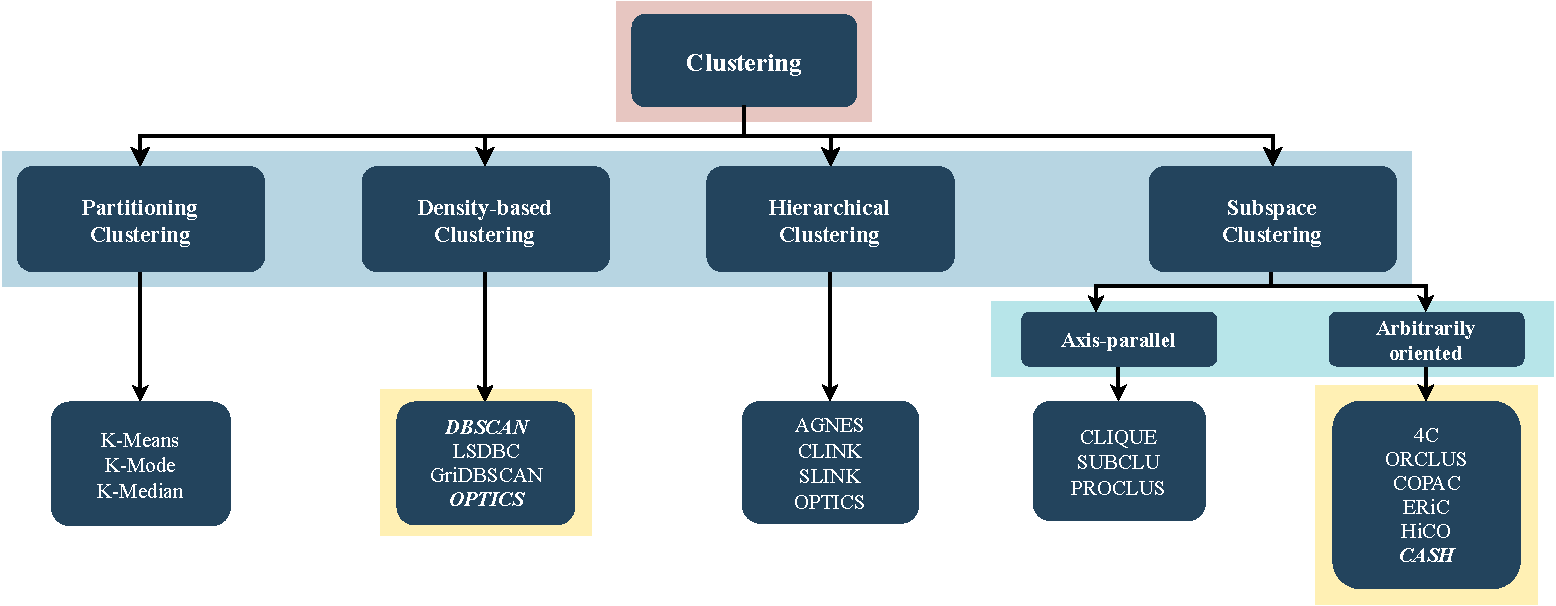
\includegraphics[width=1.1\textwidth, page=1]{figures/ClusteringAxis.pdf}}
    \caption{Topology of Clustering, Yellow marked areas are the main focus of the thesis}
    \label{fig:my_label}
\end{figure}

% source für 'basic verfahren' http://myweb.sabanciuniv.edu/rdehkharghani/files/2016/02/The-Morgan-Kaufmann-Series-in-Data-Management-Systems-Jiawei-Han-Micheline-Kamber-Jian-Pei-Data-Mining.-Concepts-and-Techniques-3rd-Edition-Morgan-Kaufmann-2011.pdf 
% source für subspace clustering verfahren: https://onlinelibrary-wiley-com.emedien.ub.uni-muenchen.de/doi/abs/10.1002/widm.1057
% lmu bookmarklet: https://www.ub.uni-muenchen.de/ausleihe-online/e-medien-login/index.html

% \section{The locality assumption}
\section{Subspace Clustering}\label{sec:subspaceclu}
